%Resume GET (parameter GET, cara penggunaan dan kode) Kelompok 3 D4TI2B
%\begin{enumerate}
%\Fikri aldi nugraha                  1164038
%\Nur Arkhamia Batubara               1164049 
%\Miftahul Hasanah                    1164046 
%\Si Made Angga Dwitya P              1164053 
%\Widary Anggraini Mindo V Siahaan    1164057
%\end{enumerate}

\section{Pengenalan Method GET Pada HTTP}
Http adalah protokol permintaan-jawaban (request-reply). Client akan mengawali koneksi dengan server dengan mengirimkan permintaan 
dengan nama dokumen yang client inginkan dan kemudian server mengirimkannya kembali dengan normal, termasuk dokumen yang diminta. http 
juga mengizinkan client untuk mengirimkan data yang diminta pengguna ke server. Http juga mengizinkan client untuk mengirimkan data 
yang diminta pengguna ke server. 

Method GET disebut juga method HTTP yang sangat sederhana dan paling banyak digunakan untuk meminta resource dari server. Method get 
memiliki banyak fungsi yaitu salah satunya digunakan untuk mengirim data diatas server, walaupun demikian hal itu memiliki batasan-
batasan. Dari seluruh karakter yang diminta kepada permintaan method GET  adalah benar - benar sangat terbatas, jadi dalam situasi ini , banyak terdapat data perlu dikirimkan ke server  dan tidak semua pesan- pesan tersebut bisa disampaikan.

HTTP mendefinisikan seperangkat metode permintaan untuk menunjukkan tindakan yang diinginkan yang akan dilakukan untuk sumber daya 
tertentu.
Meskipun mereka juga bisa menjadi kata benda, metode permintaan ini kadang-kadang disebut sebagai verba HTTP. Masing-masing menerapkan 
semantik yang berbeda, namun beberapa fitur umum digunakan bersama oleh mereka: mis. Metode permintaan dapat berupa safe, idempotent, 
atau cacheable. Salah satu metode permintaan yang digunakan dalam Http adalah GET, dimana GET ini digunakan untuk meminta representasi 
sumber atau menampilkan data/nilai pada url yang nantinya akan ditampung oleh action.

REST menggunakan protokol HTTP yang bersifat stateless. Perintah HTTP yang bisa digunakan adalah fungsi GET, POST, PUT atau 
DELETE. Hasil yang dikirimkan dari server biasanya dalam bentuk format XML atau JSON sederhana tanpa ada protokol pemaketan  
data,sehingga informasi yang diterima dapat jauh lebih mudah dibaca dan diparsing disisi client.

\section{Pengertian Method Get}
GET adalah operasi read-only yang sering digunakan untuk meminta informasi yang spesifik pada sebuah server dalam bentuk query. 
Karakteristik dari operasi GET adalah idempotent dan safe. Idempontent dapat diartikan sebanyak-banyaknya apapun operasi ini dilakukan 
dan hasilnya akan tgetap sama sedangkan, safe berarti ketika operasi ini diinvokasi tetap tidak mengubah state di server.
Biasanya GET sering ditemukan di HTML,PHP dah diterapkan juga pada Web Service.

Disamping itu Method ini juga sering diartikan juga sebagai method HTTP yang paling sederhana dan juga dapat digunakan sebagian besar 
untuk meminta mencari atau resource tertentu dari server, bisa berupa halaman web, file gambar grafis, atau sebuah dokumen , dan lain-
lain.  Di PHP method Get merupakan method dimana metode ini dapat mengirimkan informasi pengguna yang telah dikodekan dan ditambahkan 
permintaan halaman. Halaman informasi dikodekan dan dipisahkan oleh karakter tanda seru.

Web sevice merupakan layanan yang diidentifikasi dengan URI (Uniform Resource Identifier) yang mengekspos fiturnya dengan melalui 
internet dan memanfaatkan protocol, Bahasa standar internet  serta diimplementasikan menggunakan internet stantar contohnya XML. Bahasa 
pemograman php bisa digunakan dalam web service dengan memanfaatkan method seperti GET dan POST, kemudian PHP juga memiliki fungsi 
untuk mendukung pengiriman maupun pengolahan data dalam format JSON. Selain itu  agar PHP dapat mengirimkan data dalam format JSON, PHP 
menggunakan fungsi json encode.  

Dalam Bahasa PHP melakukan HTTP request ke halaman kemudian secara default adalah get request, data yang didapatkan dari web service 
dikirimkan dalam bentuk format standar misalnya XML atau JSON atau Java Object Notation. Get memiliki fungsi yang sama seperti POST 
digunakan untuk mengirimkan nilai atau value variabel ke file yang telah diatur. Perbedaan method GET dan method POST sangat kecil 
tetapi sangat terlihat dengan jelas.

Bahasa pemograman PHP dapat kita gunakan untuk membuat web service yang  berbasis kepada RPC (Remote Procedure Call) , kemudian kita 
menggunakan SOAP untuk memanggil method atau fungsi yang berbeda pada computer lain dengan menggunakan internet. Supaya client bisa 
mengetahui method yang tersedia, port, format data input output, dan keterangan lain maka harus  dideklarasikan dengan standar WSDL.    
Metode umum yang dapat digunakan oleh HTTP untuk dapat membaca data kedalam sebuha browser adalah dengan menggunakan metode get. 
Metodeget ini dirancang hanya dapat kita gunakan untuk membaca sebuah data namun dapat disayangkan secara praktek dapat digunakan juga untuk melewatkan data dengan menambahkan informasi pada sebuah URL. Maka dengan cara tersebut makametode get akan melewatkan data yang dapat dilihat oleh pengguna melalui alamat URL yang juga dapat kita simpan pada bookmark.

Metode GET pada HTTP/1.0 mempunyai batas maksimum parameter data sepanjang batas URL dengan batas ukuran maksimum 2 kb untuk browser 
saat in. HTTP/1.1 tidak memberikan batas maksimum untuk Uniform Resource Identifier (URI). Penyebutan yang lebih umum untuk URL. Metode 
lain yang dapat kita gunakan agar kita dapat  mengirimkan data yaitu kita dapat menggunakan  metode POST. Dimana metode  POST ini 
memiliki banyak kelebihan dibandingkan dengan  metode GET ,kelebihan yang dimaksud tersebut yaitu metode POST  memliki panjang 
parameter dan tidak  terbatas,  metode POST tidak dapat terlihat oleh pengguna  seperti manusia dan  kita juga tidak bias menyimpannya 
ke dalam bookmark.

\begin{figure}[ht]
\centerline{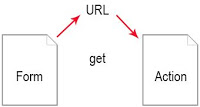
\includegraphics[width=1\textwidth]{figures/3methodget.JPG}}
\caption{Proses Kerja}
\label{proses}
\end{figure}

Contoh :
Pada gambar \ref{proses} menjelaskan tentang proses kerja.
\subsection{GET pada PHP}
GET dalam Bahasa inggris pasti kita mengenal istilah getting yang berarti mengambil, jadi bisa diartikan GET adalah metode pada HTTP 
yang digunakan untuk mengambil data dari server. pada metode ini umumnya data dbentyk dari query string yang dikirim via URL. Data yang 
dikirim tersebut berupa pasangan key sama dengan value yang dipisahkan dengan tanda dan , kemudian data tersebut digabung dengan URL 
utama yang dipisahkan dengan tanda tanya . 

Sebelum dikirim, terlebih data diproses sehingga memenuhi standar format URL. URL hanya boleh memuat huruf besar dan kecil, angka dan 
beberapa karakter lain. Karakter di luar itu akan diubah ke format tertentu yang diawali tanda persen kemudian diikuti dengan 2 digit 
hexadecimal. 
 
Angka yang terdapat pada kolom (URL Encoded) merupakan nilai yang diubah dalam bentuk hexadecimal yang didapat dari hasil character 
ASCII. Selain itu URL juga tidak boleh memuat sebuah spasi sehingga spasi akan diubah menjadi tanda tambah atau tanda persen 20. Segala proses 
tersebut disebut URL encoding, yang dilakukan untuk memenuhi standar format URL.  
 
\subsection{fungsi Method GET}
Metode umum yang digunakan HTTP untuk membaca suatu data ke dalam browser adalah metode get . Metode ini dirancang hanya 
digunakan untuk membaca data namun secara praktek digunakan juga untuk melewatkan data dengan menambahkan informasi pada URL. 
GET penggunaan untuk kelompok HTTP ini untuk mengambil atau membaca data. Method pada kelompok ini biasanya mengembalikan suatu 
keluaran atau output yang  disebut dengan function.
Fungsi GET secara teknis diproses lebih sederhana karena permintaan dikirimkan melalui alamat halaman (URL) dengan sistem 
penulisan secara berpasangan yaitu nama varibel dan nilainya, dan pemisahan variabel menggunakan karakter dan, misalnya :
\begin{verbatim}
http://localhost/obattradisional/bagian_tanaman.php
\end{verbatim}

Metode GET digunakan sehingga HTTP Client bisa mengambil informasi dari server dengan mengirimkan data melalui URI.
dan juga GET dapat digunakan untuk mengambil data dari server dan meminta sebuah respon dari resource yang spesifik.  alur dari 
metode GET akan menampilkan data/nilai pada URL, kemudian akan ditampung oleh action.Sehingga Untuk melakukan proses read pada 
pin tertentu, HTTP request yang dikirimkan harus menggunakan method GET dengan pola Request- URI.

Metode penanganan web service memakai REST dengan memakai metode GET dan pengiriman data yang dilakukan melalui URL. URL 
tersebut kemudian di-parsing dengan memakai suatu arsiterkur REST sehingga terciptalah suatu alamat URL yang universal. URL 
tersebut diuji cobakan melalui web browser, respon yang dihasilkan adalah data format XML yang berasal dari database server. 

\subsection{Karateristik dari Method GET}
Metode get juga dapat diartikan sebagai metode pengiriman data dengan menggunakan query berupa string, sehingga seluruh nilai dari form 
diitampilkan pada baris url/Address bar. Get juga dapat difungsikan sebagai penamaan (link) dalam sebuah website. Adapun beberapa 
karakteristiknya yang dimiliki oleh Get sehingga method ini bisa memudahkan user untuk melakukan pencarian data ataupun penamaan pada 
url yaitu sebagai berikut :
\begin{enumerate}
\item Variabel dapat terlihat pada url.
\item Dibatasi pada panjang string yaitu 2047 karakter.
\item Dapat memungkinkan pengunjung dapat langsung memasukkan nilai pada form variabel proses.
\end{enumerate}

\begin{table} [ht]
\caption{Karakteristik dalam bentuk tabel}
\centering
\begin {tabular} {|cc|}
\hline
a.	Method ini dapat menghasilkan string panjang yang muncul browser & \\
\hline
b.	Get tidak bisa mengirim data biner &\\
\hline
c.	Dibatasi pada panjang string yaitu 2047 karakter & \\
\hline
d.	Dapat memungkinkan pengunjung dapat langsung memasukkan Nilai & \\
\hline
\end{tabular}
\label{ltabel}
\end{table}

\subsection{Keuntungan Penggunaan Method GET}
Keuntungan dari penggunaan get tersebut adalah permintaan URl dari permintaan Get dapat juga disimpan oleh beberapa browser.
Hal itu berarti bahwa user dapat dengan mudah menyimpan permintaan dan dapat mengakses setiap saat melalui proses yang terjadi setiap 
waktunya. Hal tersebut dapat membahayakan jika penyimpanan yang dilakukan secara fungsional bukan merupakan sesuatu yang diinginkan oleh 
pengguna atau user.

Get itu sendiri dapat juga digunakan dalam pengiriman data ke server, meskipun begitu hal-hal itu mempunyai batasan. 
Jumlah dari total karakter yang dapat diubah ke dalam permintaan get adalah sangat terbatas. Sehingga untuk situasi tersebut, dimana 
banyak data-data yang perlu dikirim  ke server, tidak semua bisa pesan-pesan itu dapat disampaikan. Oleh sebab itu Get benar-benar 
sangat dibatasi dan tidak bebas.

\subsection{Kelemahan Penggunaan Method GET}
Kelemahan method GET adalah nilai dari form dapat dilihat langsung didalam URL yang dikirimkan. Jika membuat form untuk data-
data yang  sensitif seperti password. Maka form  dengan method GET bukan suatu pilihan yang bagus. Form dengan method GET 
disarankan untuk form yang berfungsi untuk menampilkan data  yaitu dimana hasil isian dari form hanya digunakan untuk  
menampilkan data.  GET dapat digunakan pada indeks yang mengambil data dari database.

\section{Batasan Dalam Get}
Batasan lain dari permintaan Get yaitu ketika mengirim data adalah data yang dikirim menggunakan method ini dan ditambahkan pada url yag 
akan dikirim ke server. Untuk itu kita dapat mengasumsikan URL sebagai alamat yang unik yang akan dikirim ke server sebagai penandan 
lokasi yang diminta. Salah satu permasalahannya lai adalah URl dari beberapa permintaan yang diinginkan ditampilkan pada bar browser ke 
beberapa browser. Hal iitu dapat diartikan, bahwa beberapa data sensitive seperti password atau informasi dapat ddilihat oleh siapapun.

\section{Parameter Get}
Dalam hal penggunaannya method GET ini memiliki suatu parameter. Jika klien menggunakan protokol HTTP pada server web untuk meminta 
sumber daya tertentu, maka klien akan mengirimkan parameter GET tertentu ke server melalui URL yang diminta. Parameter ini merupakan 
pasangan nama dan nilai yang harus memiliki kesesuaian, yang disebut pasangan nama-nilai.
Nama dan nilai ini ditambahkan ke URL dengan tanda tanya dan memberi tahu server sumber daya mana yang dimaksud. Nama dan nilai selalu dipisahkan menggunakan tanda sama dengan. Tidak hanya satu tetapi juga beberapa parameter serta seluruh daftar dapat dikirim ke server. Di sini, berbagai parameter dipisahkan menggunakan tanda dan .
\begin{verbatim}
http://www.domain.com/index.html*?name1=value1
http://www.domain.com/index.html*?name1=value1&name2=value2
\end{verbatim}

Mengambil dan mengubah Teks pada Label
Walaupun jarang terjadi atau dapat kita sebut sangat jarang terjadi tapi terkaang kita juga harus mengambil isi teks suatu label atau 
kita dapat mengganti teks pada sebuah label saat program tersebut sedang berjalan.
Untuk mengambil tekas pada label kita dapat menggunakan method Get. Sedangkan untuk menentukan teks pada label kita dapat menggunakan 
method set text. 
Method get akan dihilangkan pada GTK 2.0 dan kita dapat menggantinya dengan menggunakan get teks.

\section{Parameter Get}
Method “get”
Pada saat penggunaan method “get” dimana membolehkan input yang kita masukkan dipaparkan sama ada pada halaman yang sama atau halaman 
 yang berbeda/lainnya. Brikut merupakan contoh dari penggunaan sintaks mehod “get” yaitu”
Simpanah sintaks berikut dalam bentuk shah.asp
\begin{verbatim}
<html>
<body>
<form action=”shah.asp” method=”get”>
Nama
<input type=”submit” value=”Submit”>
</form>
<%
Dim fname
Fname=Request.QueryString(“fname”)
If fname<>”” Then
Response.Write(“Hai” & fname &  “!<br> />”)
Response.Write(“Apa khabar hari ini ?”)
End if
%>
</body>
</html>
\end{verbatim}

Dari contoh diatas menunjukkan contoh kemasukan data. Dimana kita hanya perlu memasukkan nama anda pada ruangan input. Setelah itu kita 
akan mengklik button submit.

\subsection{Properi kontrol pada object data source}
1.	DataObject Type nama = get atau set nama class yang digunakan kontrol Object Data Source sebagai parameter untuk update insert atau 
delete operasi data.
2.	Delete Method = get atau set method middle tier yang digunakan kontrol object Data Source untuk menghapus data dari database.
3.	Delete Parameters = get collection parameter yang digunakan oleh metod yang terdapat di property delete method.

\section{Penggunaan Get}
Antarmuka antara pengguna dan browser adalah bahasa HTML yang terstandarisasi. Sedangkan komunikasi antara browser dan server 
menggunakan protokol HTTP. HTTP juga disebut protokol client/server, dengan arti bahwa browser adalah client dan server Web adalah 
server. Pada protokol HTTP, sebuah server biasanya menunggu permintaan client. 
Contoh sederhana dari permintaan client adalah sebagai berikut.
\begin{verbatim}
GET /index.php HTTP/1.1
HOST : www.google.com
\end{verbatim}
Keterangan:
\begin{enumerate}
\item GET adalah metode HTTP yang digunakan untuk mengambil kembali halaman (retrive).
\item index.php adalah file yang diambil kembali.
\item HTTP 1.1 adalah versi dari protokol, yaitu browser yang digunakan.
\item www.google.com adalah nama host server.
\end{enumerate}
Selain itu di dalam PHP saat akan mengirimkan sebuah data dari form isian kepada server, digunakan juga method yang berfungsi untuk 
menjelaskan bagaimanadata isian form akan dikirim oleh web browser. Nilai dari method ini dapat berupa GET. 
Jika menggunakan method GET maka isian form akan ditampilkan pada url browser. Method GeT biasanya digunakan untuk data yang bersifat 
tidak rahasia seperti query pencarian. 

\subsection{Pengiriman Antar halaman Web}
Taf <FORM> memilki antribut bernama method yang digunakan untuk menentukan metode pengirimana apa yang akan kita gunakan. Salah satu 
metode yang dapat kita gunakan adalah metode get dimana metode get ini , maka setiap nilai nilai yang kita masukkan kedalam form yang 
kita kirimkan akan tampak pada address bar.Dalam php jika kita melakukan pengiriman dengan menggunakan metode get maka pada halaman web 
si penerima akan dugunakan variabel array bernama GET untuk menangkapnya.

